\documentclass[t]{beamer}

\mode<presentation>
{
  \usetheme{default}
  \setbeamertemplate{navigation symbols}{}
  \setbeamertemplate{footline}[frame number]
  \setbeamertemplate{items}[circle]
  \usecolortheme{seahorse}
}

\usepackage[english]{babel}
\usepackage[utf8]{inputenc}
\usepackage{times}
\usepackage[T1]{fontenc}
\usepackage{url}
\usepackage{amsmath}

\parskip=8 pt

\newcommand\topstrut{\rule{0pt}{2.6ex}}
\newcommand\bottomstrut{\rule[-1.2ex]{0pt}{0pt}}
\newcommand\doublestrut{\rule[-1.2ex]{0pt}{3.6ex}}

\newcommand\blue[1]{\textcolor{blue}{#1}}
\newcommand\red[1]{\textcolor{red}{#1}}
\newcommand\gray[1]{\textcolor{gray}{#1}}
\newcommand\smallgray[1]{\textcolor{gray}{\small\it #1}}
\newcommand\prevwork[1]{\smallgray{#1}}

% The differential in an integral.
% After a function or a fraction, the \, may not be desired, see \DD.
% It is as much art, taste, and consistency as norms and science.
\newcommand\D[1]{\,\mathrm{d}{#1}}
\newcommand\DD[1]{\mathrm{d}{#1}}
\newcommand\E[0]{\mathbf{E}}
\newcommand\var[0]{\mathbf{Var}}
\newcommand\N[0]{\mathcal{N}}
\newcommand\R[0]{\mathbb{R}}

\title
{Statistics for Machine Learning and Big Data}
\subtitle{An Introduction}

\author[Abrahamson] {Jeff Abrahamson}

% If you wish to uncover everything in a step-wise fashion, uncomment
% the following command: 
%\beamerdefaultoverlayspecification{<+->}

\begin{document}

\begin{frame}
  \titlepage
\end{frame}

\begin{frame}
  \frametitle{Useful facts}

  \vfill
  \only<1>{\centerline{I am a computer scientist.}}
  \only<2>{\centerline{Python is a useful tool.}}
  \vfill

  \note{
    My goal is to understand computer science and machine learning.

    Our goal this week is to understand statistics and to use python
    to help us.  Not to learn anything in particular about python.
  }
\end{frame}

\section{Probability}

\begin{frame}
  \frametitle{Review}
  \begin{itemize}
  \item Counting
  \item Urns (sampling)
  \item Area
  \end{itemize}
\end{frame}

\begin{frame}
  \frametitle{Words}

  \begin{itemize}
  \item Disjoint (mutually exclusive)
  \item Complement of an event (set)
  \item Independence
  \item Conditional probability
  \item Marginal probability
  \item Joint probability
  \end{itemize}

  \note {
    Addition rule:  We can add probabilities if the events are
    disjoint: $\Pr(A\cup B) = \Pr(A) + \Pr(B)$.

    General addition rule:  Think of Venn diagrams.
    \begin{displaymath}
      \Pr(A\cup B) = \Pr(A) + \Pr(B) - \Pr(A\cap B)
    \end{displaymath}

    Two events are independent of knowing the outcome of one gives no
    useful information about the outcome of the other and vice versa.

    Multiplication rule for independent processes: $\Pr(A\cap B) =
    \Pr(A) \Pr(B)$

    \textbf{Conditional probability} means prior is a smaller space, so just
    normalise to the smaller space.

    Said differently, \textbf{conditional probability} $\Pr(A\mid B)$ is the
    probability of some event $B$ conditioned on some event $A$.

    The \textbf{marginal probability} is when we don't condition.
    It's just a single variable, but implicitly there are other
    variables.

    \textbf{Joint probability} is taking multiple variables into
    account together.

    So general multiplication rule: $\Pr(A\cap B) = \Pr(A\mid B)
    \Pr(B)$.

    TODO: Show addition and multiplication rules somewhere here.
  }
\end{frame}

\begin{frame}
  \frametitle{Conditional Probability}

  TODO

  Side by side minipage: figure and equation

  \begin{displaymath}
    \Pr(A\mid B) = \frac{\Pr(A\cap B)}{\Pr(B)}
  \end{displaymath}
  First show plot, then show equation, then highlight $B$, then
  highlight intersection, then highlight none.

  Then show that if $B=\cup_i B_i$, then the sum is 1 (because sum was
  $\Pr(B)$).

  Show that conditioning on an independent variable has no effect.
  Intuition, then picture, then formula with trivial cancellation.

  And then use this to show Bayes Theorem in pictures.

  \begin{displaymath}
    P(A_1 \mid B) = \frac{\Pr(B\mid A_1) \Pr(A_1)}{\Pr(B\mid A_1)\Pr(A_1) + \dots +
      \Pr(B\mid A_k)\Pr(A_k)}
  \end{displaymath}

  Go through example 2.55 from OS with comment on misleading positive
  results in rare cases.
\end{frame}

\begin{frame}
  \frametitle{Probability Density Function}

  plot

  \note { The pdf describes the distribution. }
\end{frame}

\begin{frame}
  \frametitle{Cumulative Density Function}

  plot

  \note { The cdf also describes the distribution.  It's the integral
    of the pdf.}
\end{frame}

\begin{frame}
  \frametitle{Counting}

  Example: two children, what is $P(\exists \mathrm{boy}) = P(\exists b)$?

  \only<2>{graphic of bb, bg, gb, gg with prob 1/4}
  \only<3->{graphic of bb, bg, gb, gg with prob 1/4 with circled if $\exists$ b}
  \only<4->{What about $P(\exists b \mid \exists g)$?}
  \only<5->{same graphic, fade bb, circles, show 2/3}
  \only<6->{Events have probabilities summing to 1, cover, and are disjoint.}

  \note {
    Counting:
    Count all possibilities (which are equally likely), then
    probability is the fraction of the collection.

    Random processes:

    {\it A random variable (roughly) is a variable that has some
    probability of taking on different sets of events  ($X : \Omega
    \rightarrow E$).  That use of ``probability'' is circular.  A
    random process is the time evolution of a random variable.}
  
    The probability is the proportion of times the outcome occurs if
    we observe the random process infinitely long.

    It's sometimes useful to model things as random that aren't:
    traffic, human behaviour, \dots

    Law of Large Numbers:  The larger the sample, the closer to the
    actual probability.  Still deviations, but less.

    Example:  Brownian motion.  Vacuum on one side of the room.
  }
\end{frame}

\begin{frame}
  \frametitle{Pólya urn model}

  $r$ red balls, $b$ black balls in an urn.

  \only<2->{
  \begin{itemize}
  \item Sampling with replacement and duplication (rich get richer)
  \item Variations: balls into boxes
    \begin{itemize}
    \item Sampling with replacement
    \item Sampling without replacement
    \end{itemize}
  \end{itemize}
  }
  \only<3->{Want to know sequence of colours selected, evolution of colour distribution in urn.}
\end{frame}

\begin{frame}
  \frametitle{Sampling}

  \begin{itemize}
  \item We don't know $r$, $b$, or even $r/b$.  Estimate.
  \end{itemize}

  % http://en.wikipedia.org/wiki/Simple_random_sample
  % http://en.wikipedia.org/wiki/Urn_problem
\end{frame}

\begin{frame}
  \frametitle{Area}

  \begin{itemize}
  \item Continuous case.
  \item Events are regions.
  \item Same constraints: sum of areas is unity.  Cover and disjoint.
  \item Zero probability events!
  \end{itemize}

  \note {
    Discrete:  throwing darts at a checker board.
    \begin{itemize}
    \item What's the probability of hitting a white square?
    \item P(white square in bottom left quadrant)
    \end{itemize}

    Continuous:  throwing darts at the same board but no colour borders.
    \begin{itemize}
    \item P(region with colour of reddish hue)
    \item P(region with reddish hue and within 2 cm of blue region)
    \end{itemize}
  }
\end{frame}

\begin{frame}
  \frametitle{Distributions}

  Sneak preview of some common distributions, what they look like, and processes giving rise to them.
\end{frame}


\section{Statistics}
%\subsection{Subsection}

\begin{frame}
  \frametitle{What is statistics?}
  \begin{enumerate}
  \item<1-> Identify a question or problem.
  \item<1-> Collect relevant data on the topic.
  \item<1-> Analyze the data.
  \item<1-> Form a conclusion.
  \end{enumerate}
  \only<2>{Sadly, sometimes people forget 1.}
  \only<3->{Statistics is about making 2--4 efficient, rigorous, and meaningful.}
  \only<4>{\prevwork{\textit{OpenIntro Statistics}, 2nd edition, D.~Diez, C.~Barr, M.~Çetinkaya-Rundel, 2013.}}
\end{frame}


\begin{frame}
  \frametitle{Significance}

  \begin{itemize}
  \item Flip a coin $N$ times.  Get 49\% heads.  Is the coin fair?
  \item Congress/parliament has $N$ members of whom $m$ are male.  Do
    we discriminate against women?
  \item Do we discriminate against women more or less than we
    discriminate against blacks?
  \item Email classification: spam or not?
  \item Careful about what we conclude.  Here we can't conclude
    anything about cause or source.
  \end{itemize}

  % This needs supporting slides with computations.  We'll also have
  % to come back to it when we understand about $p$ values and the
  % like.
  
\end{frame}

\begin{frame}
  \frametitle{Terminology}

  \begin{itemize}
  \item A \textbf{case} or {observational unit} is an observation or a
    single sample.  E.g., an email.
  \item A \textbf{variable} is a characteristic of an observational
    unit.  E.g., number of lines, mean line length, number of words.
  \end{itemize}
  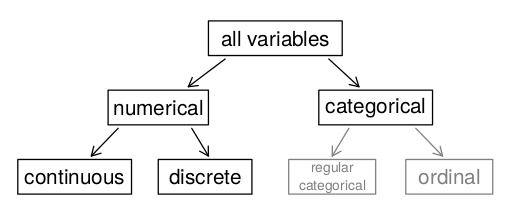
\includegraphics[width=.9\textwidth]{variable-types.png}

  Notes:  Categorical is sometimes called nominal.  Categorical
  variables with logical ordering (empty, half, full) or called ordinal.
\end{frame}

\begin{frame}
  \frametitle{Anecdote}

  Some properties of anecdote:
  
  \begin{itemize}
  \item is data
  \item haphazardly collected
  \item is generally not representative
  \item sometimes result of selective retention
  \item does not accumulate to be representative
  \item might be true (by chance)
  \item is ok to use as hypothesis, but be clear that hypothesis is anecdote
  \end{itemize}
\end{frame}

\begin{frame}
  \frametitle{Study Types}

  \begin{itemize}
  \item Observational
  \item Experimental
  \end{itemize}
  
  \note {
    
  }

  \only<2>{
    The possible gremlins:
    \begin{itemize}
    \item Association $\ne$ causation
    \item Randomness
    \item Confounding variables
    \item 
    \end{itemize}
  }
  \note {
    Example:  Sunscreen use associated with skin cancer.  But sun
    exposure is a confounding variable.

    Observational studies: prospective (identify individuals, collect
    information) and retrospective.  (Can combine the two.)
  }
\end{frame}

\begin{frame}
  \frametitle{Observational studies}

  TODO

  Can't generally conclude causation.
\end{frame}

\begin{frame}
  \frametitle{Experiment}

  We do stuff.  Maybe randomised experiment.
  
  \note{
    If well-designed, can conclude causation.

    Experiments to generate hypotheses vs experiments to demonstrate
    hypotheses.  (Don't use the same data!)

    Example: Phase 0 (10 people) and phase 1 (20-100 people) clinical trials are not randomised.

    Phase 0:  Pharmacodynamics and pharmacokinetics, particularly oral
    bioavailability and half-life of the drug.  Very small,
    subtherapeutic doses.

    Phase 1:  Testing of drug on healthy volunteers for dose-ranging.
    Often subtherapeutic, but with ascending doses.  Determine whether
    a drug is safe to check for efficacy in phase 2.
  }

  \only<2>{
    \begin{itemize}
    \item Controlling
    \item Randomisation
    \item Replication
    \item Blocking \gray{(optional, advanced)}
    \end{itemize}
  }

  \only<3>{
    \begin{itemize}
    \item $H_0$: Independent (or null) hypothesis
    \item $H_A$: Alternative hypothesis
    \end{itemize}
  }

\end{frame}

\begin{frame}
  \frametitle{Simple random sampling}

  Uniform and independent.

  \note{
    \begin{itemize}
    \item Each case has the same probability of being included.
    \item Knowing that a particular case is included provides no useful information about other cases.
    \end{itemize}

    Example: Footballers in Europe, put all the names in a bucket.
  }

  \only<2>{
    The possible gremlins:
    \begin{itemize}
    \item Not actually random
    \item Convenience sample
    \item Non-response bias
    \end{itemize}
  }

\end{frame}

\begin{frame}
  \frametitle{Stratified Sampling}

  Group like with like, then usually simple random sampling of each stratum.
  
  \note{
    Divide and conquer.

    Example:  Footballers in Europe, sample $k$ from each team.
    (Hypothesis:  footballers are paid about the same within a team.)
  }

  \only<2>{
    The guaranteed gremlin: harder to analyse than simple random sampling.
  }

\end{frame}

\begin{frame}
  \frametitle{Cluster Sampling}

  Simple random sampling to form clusters, then simple random
  sampling.

  \note{
    Example:  Sample $k$ from each village.  Works if villages have high
    diversity, not so much if villages are substantially different from
    one another.

    Example:  Ebola.  SRS expensive (census of each village, then
    maybe have to visit them all).  So select $n$ villages and sample
    $k$ within each.  Hope that villages are similar enough that this
    is valid as a first step.
  }

  \only<2>{
    The guaranteed gremlin: harder to analyse than simple random sampling.
  }
\end{frame}

\begin{frame}
  \frametitle{Mean}

  \begin{itemize}
  \item Weighted and unweighted
  \item Centroid to physicists
  \end{itemize}

  \note{
    Sample mean vs true (population) mean.
  }

  \only<2-4> {
    \centerline{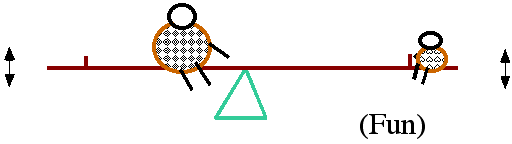
\includegraphics[width=.8\textwidth]{teeter-totter.png}}
  }
  \only<3>{
    \begin{displaymath}
      \mu = E(X) = \sum w_i x_i = \mathbf{w\cdot x}
    \end{displaymath}

    \prevwork{\url{http://telescopes.stardate.org/images/research/teeter-totter/TT4.gif}}
  }
  \only<4>{
    \begin{displaymath}
      \mu = E(X) = \sum \Pr(X=x_i) x_i
    \end{displaymath}

    \prevwork{\url{http://telescopes.stardate.org/images/research/teeter-totter/TT4.gif}}
  }
  \only<5>{
    \begin{displaymath}
      \mu = E(X) = \int xf(x) \D{x}
    \end{displaymath}

    \prevwork{\url{http://telescopes.stardate.org/images/research/teeter-totter/TT4.gif}}
  }
  \only<6>{
    \centerline{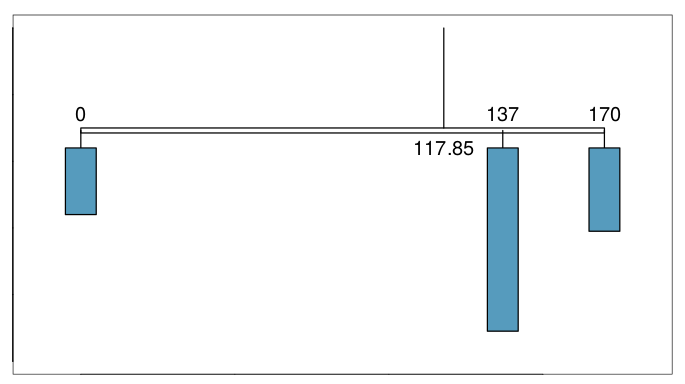
\includegraphics[width=.8\textwidth]{centroid-hanging-discrete.png}}
  }
  \only<7>{
    \centerline{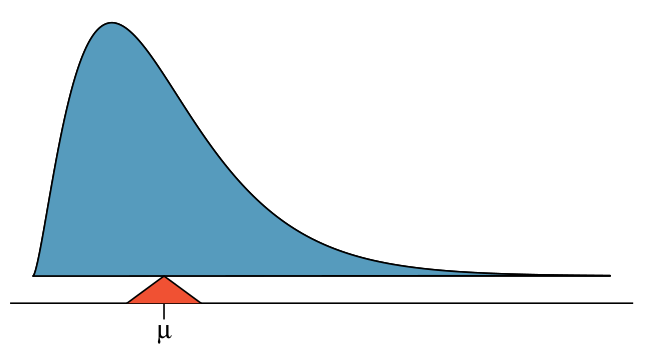
\includegraphics[width=.8\textwidth]{centroid-balance-continuous.png}}
  }
\end{frame}

\begin{frame}
  \frametitle{Variation}
  \begin{itemize}
  \item Deviation is distance from mean.
  \item Variance is mean square of deviations
  \item Standard deviation is square root of variance
  \end{itemize}
  
  \note{
    Sample standard deviation ($s$) and sample variance ($s^2$),
    divide by $n-1$.

    Population standard deviation ($\sigma$) and population variance ($\sigma^2$),
    divide by $n$.

    Population statistics may not be feasible or possible to compute.
  }

  \only<2>{
    \begin{displaymath}
      s^2 = \frac{(\overline x - x_1)^2 + \dotsb (\overline x - x_n)^2}{n-1}
    \end{displaymath}
  }
  \only<3>{
    \begin{displaymath}
      \sigma^2 = \frac{(\overline x - x_1)^2 + \dotsb (\overline x - x_n)^2}{n}
    \end{displaymath}
  }
  \only<4>{
    \begin{displaymath}
      \mbox{Var}(X) = \sigma^2 = (\overline x - x_1)^2 \Pr(X=x_1) + \dotsb
        (\overline x - x_n)^2 \Pr(X=x_n)
    \end{displaymath}
  }

\end{frame}

\begin{frame}
  \frametitle{Linear combinations of random variables}

  Assuming $X$ and $Y$ are independent:
  
  \begin{displaymath}
    \E(aX+bY) = a\E(X) + b\E(Y)
  \end{displaymath}

  \begin{displaymath}
    \var(aX+bY) = a^2\var(X) + b^2\var(Y)
  \end{displaymath}
\end{frame}

\begin{frame}
  \frametitle{Games}

  \only<1-3> {
    Multiple choice exam, 10 questions, all have four choices of which
    precisely one is correct.  Guess at random.
    \begin{itemize}
    \item Probability of getting 100\%? \only<2--5>{$\left(\frac 14\right)^{10}$}
    \item Probability of getting 0\%? \only<3--5>{$\left(\frac 14\right)^{10}$}
    \item Expected score? \only<4--5>{$10\left(\frac 14\right) = \frac
        52$}
    \item Standard deviation \only<5>{$\var(X) = \frac 14 \frac 34 = \frac 3{16}$}\only<6>{$10\left(\frac 3{16}\right) = \fr-ac {15}{8}$}
    \end{itemize}
    We'll come back to: if student gets 9 of 10 correct, do we really
    believe that they guessed at random?
  }

  \only<6> {
    
  }
  \only<7> {
    
  }

  \note{Anyone in the room worked in finance?}
  \only<8> {
    You pay \pounds 1 to turn a coin.  If it's heads, you win \pounds
    2.  If it's tails, you lose but may play again for \pounds 2.  The
    game keeps doubling: pay \pounds 2 to lose or win \pounds 4.  Pay
    \pounds 4 to lose or win \pounds 8.  Etc.
  }

\end{frame}

\begin{frame}
  \frametitle{Example: testing for rare diseases}

  A disease with incidence $D$ (i.e., probability that a randomly
  selected person has it is $D$) has a test that reliably detects
  positives (sick people) with probability $p^+$ and negatives with
  probability $p^-$.

  You test positive.  What is the probability that you have the disease?

  You test negative.  What is the probability that you have the
  disease?

  TODO: math
\end{frame}

\begin{frame}
  \frametitle{Experimental design}
  \only<1>{A telephone survey company dials digits at random (some of
    them aren't valid telephone numbers) rather than using a phone directory.
  }
  \only<2>{A statistics student wants to determine if social network
    usage among his peers (students at his school) affects academic
    performance.  Possibilities:
    \begin{itemize}
    \item He messages his class snapchat group.
    \item He posts paper fliers at his university.
    \item He gets a list of students from the registrar.  (What about
      opt-in/opt-out policies?  What if he doesn't know how many have
      opted out/failed to opt in?
    \item Other)
    \end{itemize}

  }
  \only<3>{Due to a flu epidemic, 10\% of students in a class miss the
    (final) exam.  The professor decides to offer a make-up exam but
    to require 11\% of the students who took the original exam to take
    the make-up exam as well in order to calibrate the new exam and
    make results comparable.
  }
  \only<4>{
  }
  \only<5>{
  }
  
  \note{
    Discuss.  Explain flaws.  Discuss what researcher should have done differently.
  }

\end{frame}

\begin{frame}
  \frametitle{Reasoning about data}

  \only<1>{Students at an elementary school are given a questionnaire
    that they are required to return after their parents have
    completed it. One of the questions asked is, “Do you find that
    your work schedule makes it difficult for you to spend time with
    your kids after school?” Of the parents who replied, 85\% said
    “no”. Based on these results, the school officials conclude thata
    great majority of the parents have no difficulty spending time
    with their kids after school.
  }
  \only<2>{A survey is conducted on a simple random sample of 1,000
    women who recently gave birth, asking them about whether or not they
    smoked during pregnancy. A follow-up survey asking if the children
    have respiratory problems is conducted 3 years later, however, only
    567 of these women are reached at the same address. The researcher
    reports that these 567 women are representative of all mothers.
  }
  \only<3>{An orthopedist administers a questionnaire to 30 of his
    patients who do not have any joint problems and finds that 20 of
    them regularly go running. He concludes that running decreases the
    risk of joint problems.
  }
  \only<4>{
  }
  \only<5>{
  }

  \note{
    Explain flaws.  Discuss what researcher should have done differently.
  }
  
\end{frame}

\begin{frame}
  \frametitle{Example}

  \centerline{Mammals}

  \centerline{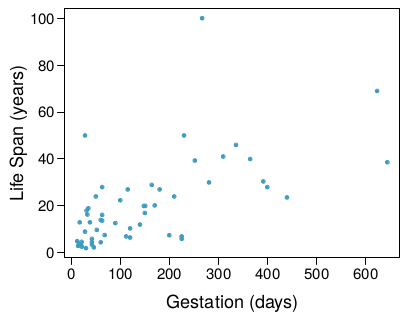
\includegraphics[width=.8\textwidth]{mammal-gestation.png}}

  \note{
    Discuss.  Are the variables independent?
  }
  
\end{frame}

\section{Distributions}

\begin{frame}
  \frametitle{Bernoulli distribution}

  Takes value 1 with probability $p$ and 0 with probability $1-p$.
  \bigskip
  
  \begin{tabular}{ll}
    Model & turning coins\\[1mm]
    Parameters & $p\in [0,1]$\\[1mm]
    Mean & $p$\\[1mm]
    Variance & $p(1-p)$
  \end{tabular}

  TODO: need a picture of pdf, cdf
  
  \note{

  }
  
\end{frame}

\begin{frame}
  \frametitle{Poisson distribution}

  Probability of a given number of events occurring in a fixed
  interval of time and/or space if these events occur with a known
  average rate and independently of the time since the last event.
  \bigskip
  
  \begin{tabular}{ll}
    Model & radioactive decay, network packets\\[1mm]
    Parameters & $\lambda\in \R^+$\\[1mm]
    Mean & $\lambda$\\[1mm]
    Variance & $\lambda$
  \end{tabular}

  TODO: need a picture of pdf, cdf
  
  \note{

  }
  
\end{frame}

\begin{frame}
  \frametitle{Binomial distribution}

  $\mathbf{B}(n,p) = $ Number of successes in a sequence of $n$ independent bernoulli
  trials (yes/no experiments), each of which yields success with
  probability $p$.
  \bigskip

  \begin{tabular}{ll}
    Model & sequences of coin tosses\\[1mm]
    Parameters & $n$, $p$\\[1mm]
    Mean & $np$\\[1mm]
    Variance & $np(1-p)$
  \end{tabular}

  TODO: Pictures of pdf, cdf.
  
  \note{

  }
  
\end{frame}

\begin{frame}
  \frametitle{Normal distribution}

  $\N(\mu,\sigma^2)$, about which we will say a great deal over the
  next hour and the rest of the day.
  \bigskip
  
  \begin{tabular}{ll}
    Model & cf. CLT\\[1mm]
    Parameters & $\mu$, $\sigma^2$\\[1mm]
    Mean & $\mu$\\[1mm]
    Variance & $\sigma^2$
  \end{tabular}

  TODO: Pictures of pdf, cdf.
  \note{
    Note that unimodal and roughly symmetric does not necessarily mean normal.
  }
  
\end{frame}

\begin{frame}
  \frametitle{}

  \note{

  }
  
\end{frame}

\begin{frame}
  \frametitle{}

  \note{

  }
  
\end{frame}

\begin{frame}
  \frametitle{}

  \note{

  }
  
\end{frame}

\begin{frame}
  \frametitle{}

  \note{

  }
  
\end{frame}

\begin{frame}
  \frametitle{}

  \note{

  }
  
\end{frame}

\begin{frame}
  \frametitle{}

  \note{

  }
  
\end{frame}

\begin{frame}
  \frametitle{}

  \note{

  }
  
\end{frame}

\begin{frame}
  \frametitle{}

  \note{

  }
  
\end{frame}

\begin{frame}
  \frametitle{}

  \note{

  }
  
\end{frame}

\begin{frame}
  \frametitle{}

  \note{

  }
  
\end{frame}

\begin{frame}
  \frametitle{}

  \note{

  }
  
\end{frame}

\begin{frame}
  \frametitle{Questions?}
  \vspace{3cm}
  \centerline{\large\url{purple.com/talk-feedback}}
\end{frame}


\end{document}

%% ToDo:
%%
%%   Box plots
%%   Side-by-side box plots
%%   Hollow histograms
%%   Robust vs non-robust statistics (cf. log. p. 30 / phys. p. 40 in OS)
%%   Example: non-random sample before U.S. presidential, company tanked
%%     (rise of Nielson?)
%%   Example: 4 distributions with same mean, std dev
%%   
%%   Visualisation and intuition
%%   http://xkcd.com/552/
%%
%%   Tufte space shuttle data/visualisation
%%   Marathon time plots (OS, physical 70)
